\documentclass[11pt,a4paper]{article}

% Overleaf compiler: pdfLaTeX
\usepackage[utf8]{inputenc}
\usepackage[T1]{fontenc}
\usepackage{lmodern}
\usepackage[a4paper,margin=0.8in,headheight=39pt,headsep=14pt,footskip=25pt]{geometry}
\usepackage{amsmath,amssymb}
\usepackage{array,booktabs,tabularx}
\usepackage{enumitem}
\usepackage{fancyhdr}
\usepackage{graphicx}
\usepackage{adjustbox}
\usepackage{microtype}
\usepackage{xcolor}
\usepackage{tikz}
\usepackage[font=small,labelfont=bf]{caption}
\usetikzlibrary{arrows.meta,positioning,calc,shapes.geometric,fit,trees}

\definecolor{navy}{RGB}{31,78,121}
\definecolor{paleBlue}{RGB}{229,237,247}
\definecolor{paleGray}{RGB}{245,246,248}

% Edit this single definition to change the roll number throughout the document.
\newcommand{\RollNumber}{24118105}
\newcommand{\StudentName}{Shourya Veer Singh}

\setlength{\parindent}{0pt}
\setlength{\parskip}{2pt}
\setlist[itemize]{leftmargin=1.4em,itemsep=1pt,topsep=1pt}
\setlist[enumerate]{leftmargin=1.6em,itemsep=1pt,topsep=1pt}
\renewcommand{\arraystretch}{1.08}
\raggedbottom

\pagestyle{fancy}
\fancyhf{}
\fancyhead[R]{%
  \begin{tabular}{@{}r@{}}
    \small\textbf{Name: \StudentName}\\[-1pt]
    \small Roll No.: \RollNumber\\[-1pt]
    \small Signature: \rule{2.2cm}{0.4pt}
  \end{tabular}}
\fancyfoot[C]{\small ITC Assignment 01}
\fancyfoot[R]{\small\thepage}
\renewcommand{\headrulewidth}{0.4pt}
\renewcommand{\footrulewidth}{0pt}
\fancypagestyle{plain}{%
  \fancyhf{}
  \fancyhead[R]{%
    \begin{tabular}{@{}r@{}}
      \small\textbf{Name: \StudentName}\\[-1pt]
      \small Roll No.: \RollNumber\\[-1pt]
      \small Signature: \rule{2.2cm}{0.4pt}
    \end{tabular}}
  \fancyfoot[C]{\small ITC Assignment 01}
  \fancyfoot[R]{\small\thepage}
  \renewcommand{\headrulewidth}{0.4pt}
}
\fancypagestyle{cover}{%
  \fancyhf{}
  \fancyhead[R]{%
    \begin{tabular}{@{}r@{}}
      \small\textbf{Name: \StudentName}\\[-1pt]
      \small Roll No.: \RollNumber\\[-1pt]
      \small Signature: \rule{2.2cm}{0.4pt}
    \end{tabular}}
  \fancyfoot[C]{\small ITC Assignment 01}
  \renewcommand{\headrulewidth}{0.4pt}
  \renewcommand{\footrulewidth}{0pt}
}

\tikzset{
  block/.style={draw=navy,fill=paleBlue,rounded corners=2pt,
    minimum height=8mm,text width=24mm,inner sep=1pt,align=center,font=\small},
  smallblock/.style={draw=navy,fill=paleBlue,rounded corners=2pt,
    minimum height=7mm,text width=19mm,inner sep=1pt,align=center,font=\scriptsize},
  sum/.style={draw=navy,circle,minimum size=7mm,inner sep=0pt,font=\small},
  arrow/.style={-{Stealth[length=2mm]},thick,draw=navy},
  link/.style={thick,draw=navy},
  treenode/.style={circle,draw=navy,fill=paleBlue,inner sep=2pt,
    minimum size=7mm,font=\scriptsize,align=center},
  leafnode/.style={rectangle,draw=navy,fill=paleBlue,rounded corners=1pt,
    inner sep=2.5pt,font=\scriptsize,align=center}
}

\newenvironment{scaledtikz}
  {\begin{adjustbox}{width=0.92\linewidth,keepaspectratio}\begin{tikzpicture}}
  {\end{tikzpicture}\end{adjustbox}}
\newcommand{\DiagramStart}{\begin{scaledtikz}}
\newcommand{\qheading}[1]{\par\addvspace{5pt}\noindent{\large\bfseries\color{navy}#1}\par\nobreak\smallskip}
\newcommand{\topic}[1]{\par\smallskip\noindent{\bfseries\color{navy}#1.}\enspace}

\begin{document}

\begin{titlepage}
\thispagestyle{cover}
\vspace*{1.2cm}
\begin{center}
{\Large\bfseries NATIONAL INSTITUTE OF TECHNOLOGY RAIPUR\par}
\vspace{0.35cm}
{\large Department of Information Technology\par}
\vspace{1.1cm}
{\LARGE\bfseries ASSIGNMENT 01\par}
\vspace{0.45cm}
{\large Course: ITC\par}
{\large B.Tech. -- Fifth Semester\par}
\vfill
\end{center}
\begin{center}
\renewcommand{\arraystretch}{1.6}
\begin{tabular}{|>{\bfseries}p{4cm}|p{8cm}|}
\hline
Name & \StudentName\\ \hline
Roll Number & \RollNumber\\ \hline
Signature & \rule{5cm}{0.4pt}\\ \hline
\end{tabular}
\end{center}
\vfill
\end{titlepage}
\setcounter{page}{1}

\qheading{Q1. Fundamental Principles of Data Compression}

\topic{Purpose and redundancy}
Compression represents data with fewer bits to reduce storage, bandwidth, and transmission time while preserving exact content (lossless) or acceptable quality (lossy). It exploits coding/statistical redundancy (non-uniform symbol probabilities), inter-symbol correlation, spatial redundancy (similar neighbouring pixels), and temporal redundancy (similar video frames).

\topic{Lossless and lossy methods}
Lossless coding reconstructs the source exactly and suits text, executable files, medical records, and archives; methods include RLE, Huffman, arithmetic, and dictionary coding (LZ77/LZ78/LZW). Lossy coding discards less perceptually important information in images, audio, and video; JPEG, MPEG, MP3, and AAC trade quality against size and complexity.

\topic{Compression ratio and efficiency}
Compression ratio and percentage saving are
\[
C_R=\frac{\text{original size}}{\text{compressed size}}.
\]
\[
\text{Percentage saving}=100\left(1-\frac{\text{compressed size}}{\text{original size}}\right).
\]
For symbol probabilities \(p_i\), entropy and coding efficiency are
\[
H(S)=-\sum_i p_i\log_2 p_i,\qquad
\eta=\frac{H(S)}{L_{\text{avg}}}.
\]
Entropy is the theoretical lower bound on average bits per symbol for a uniquely decodable code; efficiency approaches 100\% as \(L_{\text{avg}}\) approaches \(H(S)\).

\topic{Text-coding approaches}
Statistical codes (Huffman) shorten frequent symbols; arithmetic coding maps a message to an interval in \([0,1)\); dictionary codes replace repeated strings (LZ77 sliding window; LZ78/LZW dictionaries); RLE encodes repeated runs and is most useful after suitable preprocessing.

\qheading{Q2. Static Huffman Coding}

\topic{Working Principle}
Frequencies are known before encoding. Repeatedly merge the two least-weight nodes until one tree remains; label branches 0/1 and read each code along its root-to-leaf path.

\topic{Construction}
Initial weights: \(E=10,C=15,D=15,B=20,A=40\). Merges: \(E+D=25\), \(C+B=35\), \(25+35=60\), and \(60+A=100\).

\topic{Huffman Tree}
\begin{figure}[htbp]
\centering
\resizebox{0.82\linewidth}{!}{%
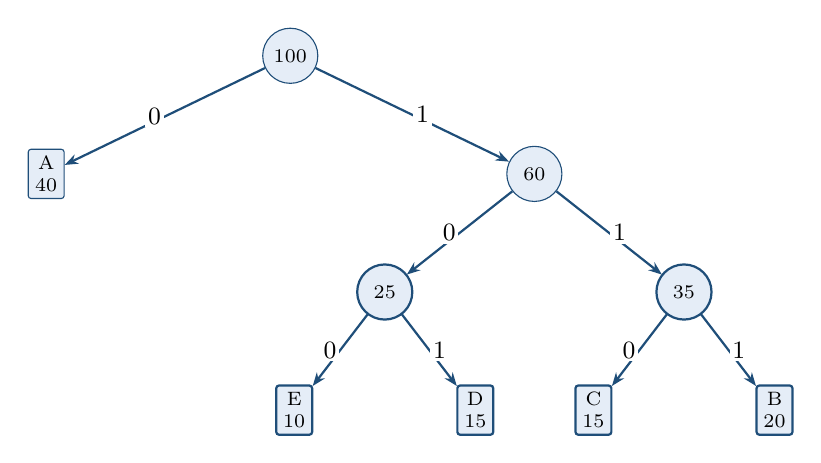
\begin{tikzpicture}[level distance=15mm,
  level 1/.style={sibling distance=62mm},
  level 2/.style={sibling distance=38mm},
  level 3/.style={sibling distance=23mm},
  edge from parent/.style={draw=navy,thick,-{Stealth[length=1.7mm]}},
  every node/.style={font=\small}]
\node[treenode] {100}
  child { node[leafnode] {A\\40}
    edge from parent node[left,draw=none,fill=white,inner sep=1pt] {0} }
  child { node[treenode] {60}
    child { node[treenode] {25}
      child { node[leafnode] {E\\10}
        edge from parent node[left,draw=none,fill=white,inner sep=1pt] {0} }
      child { node[leafnode] {D\\15}
        edge from parent node[right,draw=none,fill=white,inner sep=1pt] {1} }
      edge from parent node[left,draw=none,fill=white,inner sep=1pt] {0} }
    child { node[treenode] {35}
      child { node[leafnode] {C\\15}
        edge from parent node[left,draw=none,fill=white,inner sep=1pt] {0} }
      child { node[leafnode] {B\\20}
        edge from parent node[right,draw=none,fill=white,inner sep=1pt] {1} }
      edge from parent node[right,draw=none,fill=white,inner sep=1pt] {1} }
    edge from parent node[right,draw=none,fill=white,inner sep=1pt] {1} };
\end{tikzpicture}}
\caption{Static Huffman tree for the given symbol frequencies.}
\label{fig:huffman-tree}
\end{figure}
Therefore, the tree shown gives \(A=0\), \(E=100\), \(D=101\), \(C=110\), and \(B=111\). Codes are prefix-free: no codeword is the prefix of another.

\begin{center}
\begin{tabular}{c|c|c|c}
\toprule
Symbol & Frequency & Code & Code length\\
\midrule
A & 40 & 0 & 1\\
B & 20 & 111 & 3\\
C & 15 & 110 & 3\\
D & 15 & 101 & 3\\
E & 10 & 100 & 3\\
\bottomrule
\end{tabular}
\end{center}

\topic{Average Code Length}
\[
\begin{aligned}
L_{\text{avg}}
&=\frac{40}{100}(1)+\frac{20}{100}(3)+\frac{15}{100}(3)
 +\frac{15}{100}(3)+\frac{10}{100}(3)\\
&=0.40+0.60+0.45+0.45+0.30\\
&=2.20\ \text{bits/symbol}.
\end{aligned}
\]

\topic{Total Bits}
The source contains 40 A, 20 B, 15 C, 15 D, and 10 E symbols. Total bits:
\[
40(1)+20(3)+15(3)+15(3)+10(3)=220\ \text{bits}.
\]

\topic{Entropy and Efficiency}
The entropy of this distribution is
\[
H=-\left(0.40\log_2 0.40+0.20\log_2 0.20
+2(0.15\log_2 0.15)+0.10\log_2 0.10\right)
\approx 2.146\ \text{bits/symbol}.
\]
Efficiency is \(H/L_{\text{avg}}\approx2.146/2.20=97.6\%\). Equal-weight tie choices may change individual codes, but not the optimal average length.

\qheading{Q3. Dynamic Huffman Coding}

\topic{Concept}
Adaptive Huffman coding needs no prior frequency table: encoder and decoder start with a NYT (Not-Yet-Transmitted) node and update the same tree after every symbol.

\topic{Tree Construction and Update}
For a first occurrence, send the NYT code plus the symbol identifier and add a leaf; later occurrences use the current leaf code. Increment weights and reorder while preserving the sibling/numbered-node property (FGK or Vitter).

\begin{figure}[htbp]
\centering
\DiagramStart
\node[block] (find) at (0,0) {Read next symbol\\and find leaf/NYT};
\node[block] (emit) at (3.4,0) {Transmit current\\code (or NYT + symbol)};
\node[block] (inc) at (6.8,0) {Increment weight\\and update tree};
\node[block] (sync) at (10.2,0) {Decoder mirrors\\the same update};
\draw[arrow] (find)--(emit);
\draw[arrow] (emit)--(inc);
\draw[arrow] (inc)--(sync);
\draw[arrow] (sync.south) -- ++(0,-0.65) -| (find.south);
\node[font=\scriptsize] at (0.7,-2.5) {First symbol:};
\node[leafnode] (nyt0) at (2.6,-2.5) {NYT};
\node[treenode] (root1) at (7,-2.0) {1};
\node[leafnode] (nytl) at (6,-3.1) {NYT};
\node[leafnode] (a1) at (8,-3.1) {A\\1};
\draw[arrow] (nyt0.east)--node[above,font=\scriptsize] {new A}(root1.west);
\draw[arrow] (root1)--node[left,font=\scriptsize] {0}(nytl);
\draw[arrow] (root1)--node[right,font=\scriptsize] {1}(a1);
\node[font=\scriptsize] at (7,-3.7) {Updated tree};
\end{scaledtikz}
\caption{Adaptive Huffman update flow and example NYT tree insertion.}
\label{fig:adaptive-huffman}
\end{figure}

\topic{Update Process}
Increment the symbol leaf and update ancestors; swap only with a permitted highest-numbered equal-weight node. The decoder mirrors the update to stay synchronized.

\topic{Comparison}
Static Huffman requires known frequencies and usually a counting pass plus a tree/header; dynamic coding adapts in one pass without a complete initial table, at the cost of tree-update work and greater synchronization sensitivity.

\begin{center}
\begin{tabularx}{\linewidth}{>{\bfseries}p{0.22\linewidth}XX}
\toprule
Property & Static Huffman & Dynamic Huffman\\
\midrule
Statistics & Known before encoding & Updated as symbols arrive\\
Passes & Usually frequency pass, then encode & One pass with synchronized updates\\
Side information & Header or agreed model needed & No complete frequency table required initially\\
Adaptation & Does not adapt to changing statistics & Adapts during coding\\
Cost & Simpler tree operation & More memory and update processing\\
\bottomrule
\end{tabularx}
\end{center}

\topic{Applications}
Use static coding for known or stable distributions; dynamic coding suits streams with unknown or changing statistics.

\qheading{Q4. Arithmetic Coding}

\topic{Principle}
Arithmetic coding maps the whole message to a subinterval of \([0,1)\), refining it in proportion to symbol probabilities. For \(A=[0,0.5)\), \(B=[0.5,0.8)\), \(C=[0.8,1)\), encode ABCA as follows.

\topic{Interval Calculation}
For current interval \([L,U)\), width \(W=U-L\), and next-symbol cumulative range \([L_s,U_s)\):
\[
L'=L+W L_s,\qquad U'=L+W U_s.
\]
\[
\begin{array}{ll}
\text{Start:} & [0,1),\quad \text{width}=1.\\
A: & [0,0.5),\quad \text{width}=0.5.\\
B: & [0+0.5(0.5),\,0+0.5(0.8))=[0.25,0.40),\quad
      \text{width}=0.15.\\
C: & [0.25+0.15(0.8),\,0.25+0.15(1.0))=[0.37,0.40),\quad
      \text{width}=0.03.\\
A: & [0.37+0.03(0),\,0.37+0.03(0.5))=[0.37,0.385),\quad
      \text{width}=0.015.
\end{array}
\]
\begin{figure}[htbp]
\centering
\DiagramStart
\draw[link] (0,0)--(10,0);
\foreach \x in {0,2.5,3.7,3.85,4,5,8,10}
  {\draw[link] (\x,0.08)--(\x,-0.08);}
\foreach \x/\lab in {0/0,2.5/0.25,5/0.5,8/0.8,10/1.0}
  {\node[below=2pt,font=\scriptsize] at (\x,-0.08) {\lab};}
\draw[line width=4pt,navy] (0,0.55)--(5,0.55);
\node[above,font=\scriptsize] at (2.5,0.58) {A: [0,0.5)};
\draw[line width=4pt,red!70!black] (2.5,1.0)--(4,1.0);
\node[above,font=\scriptsize] at (3.25,1.03) {B: [0.25,0.40)};
\draw[line width=4pt,green!50!black] (3.7,1.45)--(4,1.45);
\node[right,font=\scriptsize,inner sep=1pt] at (4,1.45) {C: [0.37,0.40)};
\draw[line width=4pt,orange!80!black] (3.7,1.9)--(3.85,1.9);
\node[right,font=\scriptsize,inner sep=1pt] at (3.95,1.9) {A: [0.37,0.385)};
\draw[dashed,gray] (3.7,0.1)--(3.7,2.1);
\draw[dashed,gray] (3.85,0.1)--(3.85,2.1);
\end{scaledtikz}
\caption{Nested intervals for arithmetic encoding of ABCA.}
\label{fig:arithmetic-intervals}
\end{figure}

\topic{Final Encoded Value}
Choose the midpoint of the final interval:
\[
\frac{0.37+0.385}{2}=0.3775.
\]
The midpoint \(0.3775\in[0.37,0.385)\) identifies ABCA given the model and message length/termination convention.

\topic{Comparison with Huffman Coding}
Huffman assigns integer-length symbol codes and is simple; arithmetic coding can approach entropy more closely for skewed probabilities by coding a whole sequence. It is more complex and uses finite-precision scaling/renormalization for long messages.

\qheading{Q5. Image Compression; GIF and TIFF}

\topic{Need and Basic Principles}
Image compression exploits spatial similarity, limited palettes, and perceptually insignificant detail to reduce storage and transmission while retaining required quality.

\begin{figure}[htbp]
\centering
\DiagramStart
\node[block] (image) at (0,0) {Image samples\\and redundancy};
\node[block] (analysis) at (3.6,0) {Represent / transform\\and encode};
\node[block] (file) at (7.2,0) {Compressed image\\file};
\node[block] (display) at (10.8,0) {Decode for\\display / print};
\draw[arrow] (image)--(analysis);
\draw[arrow] (analysis)--(file);
\draw[arrow] (file)--(display);
\end{scaledtikz}
\caption{General image compression and reconstruction workflow.}
\label{fig:image-compression}
\end{figure}

\topic{GIF}
GIF is a lossless indexed-colour format (up to 256 colours) using LZW; it supports interlacing, transparency, and animation. It is compact and widely supported for flat graphics, but its palette limits photographic colour, complex images may remain relatively large, and there is little quality control.

\topic{TIFF}
TIFF is a flexible tagged raster format supporting RGB, greyscale, palette, CMYK, varied bit depths, multipage data, and metadata. It supports lossless LZW, PackBits, ZIP/Deflate, or uncompressed storage (some variants use lossy JPEG); fidelity and flexibility suit scanning and print, but files and implementations can be large/complex.

\topic{GIF versus TIFF}
\begin{center}
\begin{tabularx}{\linewidth}{>{\bfseries}p{0.17\linewidth}XX}
\toprule
Property & GIF & TIFF\\
\midrule
Colour/quality & Indexed palette of at most 256 colours & RGB, greyscale, palette, CMYK, and varied bit depths\\
Compression & Commonly LZW; lossless & LZW, PackBits, ZIP/Deflate, none; some variants allow lossy JPEG\\
Capabilities & Interlacing, transparency, short animation & Multiple pages/layers, metadata, scan data\\
Advantages & Browser support, compact flat graphics, simple animation & High quality, fidelity, professional/archival use\\
Limitations & Poor for photographs and complex colour & Large files, many optional extensions, slower processing, poor web fit\\
Typical use & Logos, icons, simple diagrams, memes, animation & Scanning, medical imaging, publishing, print workflows\\
\bottomrule
\end{tabularx}
\end{center}

\qheading{Q6. Digitized Documents}

\topic{Concept}
A digitized document is a raster scan, OCR-searchable text, or hybrid PDF/TIFF for storage, access, indexing, transmission, and backup.

\topic{Conversion Process}
Scanning converts reflected light to electrical samples; sampling and quantization form pixels, cleanup/de-skew improves them, and OCR adds searchable text before PDF/TIFF packaging.

\begin{figure}[htbp]
\centering
\DiagramStart
\node[smallblock] (paper) at (0,0) {Paper page};
\node[smallblock] (scan) at (2.6,0) {Scanner optics\\and sensor};
\node[smallblock] (sample) at (5.2,0) {Sampling and\\quantization};
\node[smallblock] (process) at (7.8,0) {Image cleanup\\and de-skew};
\node[smallblock] (ocr) at (10.4,0) {OCR text layer\\and PDF/TIFF};
\draw[arrow] (paper)--(scan);
\draw[arrow] (scan)--(sample);
\draw[arrow] (sample)--(process);
\draw[arrow] (process)--(ocr);
\end{scaledtikz}
\caption{Paper-document digitization, processing, and OCR workflow.}
\label{fig:document-digitization}
\end{figure}

\topic{Image Acquisition}
Optics, sensor, and software set acquisition quality; clean optics, correct colour settings, flat pages, and controlled lighting limit noise and shadows.

\topic{Resolution}
Resolution is measured in dpi: 150--300 dpi suits office pages; fine print/archives may need 600 dpi or more. Higher resolution increases detail, storage, and processing.

\topic{Bit Depth}
Bit depth is bits per pixel component: 1-bit for binary text, 8-bit greyscale or palette, and 24-bit RGB (8 bits/channel). Greater depth improves tonal fidelity but increases size.

\topic{Image Representation}
Pages may be bilevel/greyscale bitmaps; OCR adds XML/text or a searchable PDF text layer.

\topic{Compression}
Use lossless TIFF-LZW/ZIP or PDF streams for legal, financial, archival, and OCR-critical pages; JPEG suits controlled loss, while JBIG is suited to bilevel images. Compression reduces storage and transmission cost.

\qheading{Q7. JPEG Image Compression}

\topic{Principle}
Baseline JPEG is lossy coding for continuous-tone images, exploiting spatial redundancy and reduced visual sensitivity to high-frequency detail.

\topic{JPEG Encoder Block Diagram}
\begin{figure}[htbp]
\centering
\DiagramStart
\node[smallblock] (rgb) at (0,0) {Input image\\RGB};
\node[smallblock] (ycc) at (2.25,0) {RGB to\\YCbCr};
\node[smallblock] (blocks) at (4.5,0) {8x8 blocks\\and level shift};
\node[smallblock] (dct) at (6.75,0) {2-D DCT};
\node[smallblock] (quant) at (9,0) {Quantization};
\node[smallblock] (zig) at (11.25,0) {Zigzag, RLE,\\Huffman};
\draw[arrow] (rgb)--(ycc);
\draw[arrow] (ycc)--(blocks);
\draw[arrow] (blocks)--(dct);
\draw[arrow] (dct)--(quant);
\draw[arrow] (quant)--(zig);
\node[font=\scriptsize,below=4mm of zig] {JPEG bitstream};
\end{scaledtikz}
\caption{Baseline JPEG encoder pipeline.}
\label{fig:jpeg-encoder}
\end{figure}

\topic{Color Space Conversion}
Convert RGB to luminance \(Y\) and chrominance \(C_b,C_r\); subsample chroma (often 4:2:0 or 4:2:2) because vision is more sensitive to luminance.

\topic{DCT}
Apply a 2-D DCT to each 8x8 level-shifted block; the DC coefficient represents the average and AC coefficients represent increasing spatial frequencies:
\[
F(u,v)=\frac{1}{4}C(u)C(v)
\sum_{x=0}^{7}\sum_{y=0}^{7} f(x,y)
\cos\!\left(\frac{(2x+1)u\pi}{16}\right)\,
\cos\!\left(\frac{(2y+1)v\pi}{16}\right),
\]
where \(0\leq u,v\leq7\), \(C(0)=1/\sqrt{2}\), and \(C(k)=1\) for \(k>0\).
The inverse transform reconstructs the spatial block:
\[
\widehat{f}(x,y)=\frac{1}{4}\sum_{u=0}^{7}\sum_{v=0}^{7}
C(u)C(v)F(u,v)
\cos\!\left(\frac{(2x+1)u\pi}{16}\right)\,
\cos\!\left(\frac{(2y+1)v\pi}{16}\right).
\]

\topic{Quantization}
Divide by quantization-table entries and round; larger high-frequency entries discard detail and create zeros. The table/quality factor controls the quality--size trade-off:
\[
F_q(u,v)=\operatorname{round}\!\left(\frac{F(u,v)}{Q(u,v)}\right),
\qquad
\widehat{F}(u,v)=F_q(u,v)Q(u,v).
\]
Rounding is baseline JPEG's principal lossy step.

\topic{Zigzag Scanning}
Zigzag order scans low to high frequency, concentrating trailing zeros.

\topic{Run-Length Encoding}
RLE encodes zero-run/non-zero-value pairs; End-of-Block marks the remaining zeros.

\topic{Huffman Coding}
Huffman codes the run/amplitude symbols, assigning short codes to frequent values.

\topic{Lossy versus Lossless}
Baseline JPEG cannot recover quantized loss; lossless JPEG modes, PNG, or lossless TIFF reconstruct pixels exactly.

\qheading{Q8. Differential Pulse Code Modulation (DPCM)}

\topic{Principle}
PCM quantizes each sample independently, \(x_q[n]=Q_b(x[n])\), at \(R_{\mathrm{PCM}}=bf_s\). DPCM sends the prediction error \(e[n]=x[n]-\hat{x}[n]\); correlated samples make this error smaller-range than the source.

\topic{DPCM Block Diagram}
\begin{figure}[htbp]
\centering
\DiagramStart
\node[block] (input) at (0,1.6) {Input \(x[n]\)};
\node[sum] (diff) at (2.7,1.6) {\(+/-\)};
\node[block] (quant) at (5.3,1.6) {Error\\quantizer};
\node[block] (enc) at (8,1.6) {Encoder};
\node[block] (channel) at (10.7,1.6) {Bitstream};
\node[block] (decoder) at (13.4,1.6) {Decoder};
\node[sum] (add) at (13.4,-1) {\(+\)};
\node[block] (output) at (10.4,-1) {Reconstructed\\sample};
\node[block] (pred) at (6.2,-1) {Predictor};
\draw[arrow] (input)--(diff);
\draw[arrow] (diff)--node[above,font=\scriptsize] {\(e[n]\)}(quant);
\draw[arrow] (quant)--(enc);
\draw[arrow] (enc)--(channel);
\draw[arrow] (channel)--(decoder);
\draw[arrow] (decoder.south)--(add.north);
\draw[arrow] (add.west)--(output.east);
\draw[arrow] (output.west)--(pred.east);
\draw[arrow] (pred.north) -- ++(0,1.1) -| (diff.south);
\draw[arrow] (pred.south) -- ++(0,-0.65) -| (add.south);
\end{scaledtikz}
\caption{DPCM encoder and decoder with prediction, quantization, reconstruction, and feedback.}
\label{fig:dpcm}
\end{figure}

\topic{Predictor}
Predict from past reconstructed samples (first-order example \(\hat{x}[n]=\widetilde{x}[n-1]\)); a \(p\)-tap linear predictor is
\[
\hat{x}[n]=\sum_{k=1}^{p}a_k\widetilde{x}[n-k],
\]
where \(\widetilde{x}\) denotes reconstructed samples.

\topic{Quantizer}
Quantize the prediction error and reconstruct at both ends:
\[
e_q[n]=Q(e[n]),\qquad \widetilde{x}[n]=\hat{x}[n]+e_q[n].
\]

\topic{Encoder}
Transmit the quantizer index; the decoder adds the decoded error to its matching prediction.

\topic{Advantages}
DPCM lowers the bit rate for correlated signals and is relatively simple.

\topic{Limitations}
Performance depends on the predictor and shared reconstructed history; channel or prediction errors can cause distortion, especially for poorly predictable signals.

\qheading{Q9. Adaptive Differential Pulse Code Modulation (ADPCM)}

\topic{Concept}
ADPCM adapts quantizer step size and/or predictor to follow both small and large signal variations.

\topic{ADPCM Block Diagram}
\begin{figure}[htbp]
\centering
\DiagramStart
\node[block] (input) at (0,1.6) {Input \(x[n]\)};
\node[sum] (sub) at (2.7,1.6) {\(+/-\)};
\node[block] (aq) at (5.5,1.6) {Adaptive\\quantizer};
\node[block] (enc) at (8.2,1.6) {Encoder};
\node[block] (bits) at (10.8,1.6) {Bitstream};
\node[block] (decoder) at (13.4,1.6) {Decoder};
\node[sum] (add) at (13.4,-1) {\(+\)};
\node[block] (output) at (10.4,-1) {Reconstructed\\sample};
\node[block] (pred) at (6.2,-1) {Adaptive\\predictor};
\node[block] (adapt) at (2.7,-2.8) {Step-size and\\predictor update};
\draw[arrow] (input)--(sub);
\draw[arrow] (sub)--node[above,font=\scriptsize] {prediction error}(aq);
\draw[arrow] (aq)--(enc);
\draw[arrow] (enc)--(bits);
\draw[arrow] (bits)--(decoder);
\draw[arrow] (decoder.south)--(add.north);
\draw[arrow] (add.west)--(output.east);
\draw[arrow] (output.west)--(pred.east);
\draw[arrow] (pred.north) -- ++(0,1.1) -| (sub.south);
\draw[arrow] (pred.south) -- ++(0,-0.65) -| (add.south);
\draw[arrow] (aq.south) -- ++(0,-4.0) -| (adapt.east);
\draw[arrow] (adapt.north) -- ++(0,1.5) -| (aq.south west);
\end{scaledtikz}
\caption{ADPCM encoder and decoder with synchronized step-size and predictor adaptation.}
\label{fig:adpcm}
\end{figure}

\topic{Adaptation of Step Size}
Increase \(\Delta\) for large errors/rapid changes and decrease it for small errors:
\[
e_q[n]=Q_{\Delta[n]}(e[n]),\qquad
\Delta[n+1]=F\bigl(\Delta[n],i[n]\bigr),
\]
where \(i[n]\) is the index and both ends use the same update \(F\).

\topic{Working}
Encode the prediction error with the current step size; the decoder synchronously updates its quantizer and predictor to reconstruct each sample.

\topic{PCM, DPCM, and ADPCM Comparison}
PCM is simplest but highest-rate; DPCM exploits prediction; ADPCM adds adaptation for changing speech/audio levels at increased complexity.

\begin{center}
\begin{tabularx}{\linewidth}{>{\bfseries}p{0.18\linewidth}XXX}
\toprule
Method & What is encoded & Main advantage & Main trade-off\\
\midrule
PCM & Each sample independently & Simple, predictable reconstruction & Higher bit rate\\
DPCM & Difference from predicted sample & Efficient for correlated signals & Depends on predictor and reconstructed history\\
ADPCM & Adaptively quantized prediction error & Better handling of changing signal amplitude; lower bit rates with good perceived quality & More adaptation logic and synchronization\\
\bottomrule
\end{tabularx}
\end{center}

\qheading{Q10. Adaptive Subband Coding}

\topic{Concept}
Analysis filter banks split audio into frequency bands; code each band independently according to energy and perceptual importance.

\topic{Division into Subbands}
Low/high-pass (e.g. quadrature-mirror) filtering and downsampling form subbands; a synthesis bank reconstructs them.

\topic{Adaptive Subband Coding Diagram}
\begin{figure}[htbp]
\centering
\DiagramStart
\node[block] (input) at (0,0) {Audio input};
\node[block] (analysis) at (3,0) {Analysis filter\\bank};
\node[smallblock] (low) at (6,1.5) {Low-frequency\\subband};
\node[smallblock] (mid) at (6,0) {Mid-frequency\\subband};
\node[smallblock] (high) at (6,-1.5) {High-frequency\\subband};
\node[smallblock] (q1) at (9,1.5) {Adaptive\\quantizer};
\node[smallblock] (q2) at (9,0) {Adaptive\\quantizer};
\node[smallblock] (q3) at (9,-1.5) {Adaptive\\quantizer};
\node[block] (mux) at (12,0) {Bit allocation\\and bitstream};
\draw[arrow] (input)--(analysis);
\draw[arrow] (analysis)--(low);
\draw[arrow] (analysis)--(mid);
\draw[arrow] (analysis)--(high);
\draw[arrow] (low)--(q1);
\draw[arrow] (mid)--(q2);
\draw[arrow] (high)--(q3);
\draw[arrow] (q1)--(mux);
\draw[arrow] (q2)--(mux);
\draw[arrow] (q3)--(mux);
\node[font=\scriptsize,align=center] at (9,-2.5) {Subband energy and psychoacoustic masking\\control quantizer step sizes and allocated bits};
\end{scaledtikz}
\caption{Adaptive subband analysis and independent band coding.}
\label{fig:adaptive-subband}
\end{figure}

\topic{Independent Encoding}
Code each bandwidth-appropriate subband with PCM/ADPCM; give more bits to high-energy or perceptually important bands.

\topic{Adaptive Bit Allocation}
Estimate band energy and masking, then allocate bits by distortion/perceptual weighting; weak or masked bands receive few or no bits.

\topic{Advantages}
Frequency separation reduces quantization noise and enables masking-aware bit allocation, often improving quality over wideband coding at the same rate.

\topic{Applications}
Applications include speech/audio compression, MPEG audio, and digital broadcasting.

\qheading{Q11. Delta Modulation}

\topic{Principle}
DM sends one bit/sample indicating whether input exceeds the previous reconstruction; the accumulator steps by \(\pm\Delta\):
\[
e[n]=x[n]-\widetilde{x}[n-1],\qquad
b[n]=
\begin{cases}
1,&e[n]\geq 0,\\
0,&e[n]<0,
\end{cases}
\]
\[
\widetilde{x}[n]=\widetilde{x}[n-1]+(2b[n]-1)\Delta.
\]

\topic{Delta Modulation Block Diagram}
\begin{figure}[htbp]
\centering
\DiagramStart
\node[block] (input) at (0,1.4) {Input \(x[n]\)};
\node[sum] (cmp) at (3,1.4) {\(+/-\)};
\node[block] (quant) at (5.7,1.4) {1-bit\\quantizer};
\node[block] (bits) at (8.5,1.4) {Bitstream};
\node[block] (acc) at (5.7,-1) {Accumulator\\\(+\Delta/-\Delta\)};
\node[block] (stair) at (9,-1) {Staircase\\estimate};
\draw[arrow] (input)--(cmp);
\draw[arrow] (cmp)--node[above,font=\scriptsize] {error}(quant);
\draw[arrow] (quant)--(bits);
\draw[arrow] (quant.south)--(acc.north);
\draw[arrow] (acc)--(stair);
\draw[arrow] (stair.north) -- ++(0,0.45) -| (cmp.south);
\end{scaledtikz}
\caption{One-bit delta modulator with staircase reconstruction feedback.}
\label{fig:delta-modulation}
\end{figure}

\topic{Working}
The accumulator adds \(+\Delta\) or \(-\Delta\), forming a staircase approximation.

\topic{Slope Overload Distortion}
When input slope exceeds the maximum tracking slope \(\Delta/T_s\), the staircase falls behind: slope-overload distortion.

\topic{Granular Noise}
An overly large \(\Delta\) makes the staircase oscillate around a slowly varying signal (granular noise); a larger step reduces slope overload but worsens this noise.

\topic{Adaptive Delta Modulation}
ADM increases \(\Delta\) for consecutive same-direction bits and decreases it for alternating bits:
\[
\Delta[n+1]=
\begin{cases}
\alpha\Delta[n],&\text{for a run of same-direction bits},\\
\beta\Delta[n],&\text{for alternating bits},
\end{cases}
\qquad \alpha>1,\quad 0<\beta<1.
\]
Practical systems bound \(\Delta\) and specify the update table.

\begin{figure}[htbp]
\centering
\DiagramStart
\node[block] (bits) at (0,0) {Recent output\\bit pattern};
\node[block] (adapt) at (4,0) {Step-size\\adaptation logic};
\node[block] (delta) at (8,0) {Adaptive\\\(\Delta[n]\)};
\node[block] (acc) at (12,0) {Accumulator\\and estimate};
\draw[arrow] (bits)--(adapt);
\draw[arrow] (adapt)--(delta);
\draw[arrow] (delta)--(acc);
\node[font=\scriptsize,align=center,text width=5cm] at (6,-1.0) {Repeated same-direction bits increase \(\Delta\); alternating bits decrease \(\Delta\).};
\end{scaledtikz}
\caption{Adaptive delta modulation step-size control.}
\label{fig:adaptive-delta}
\end{figure}

\topic{DM versus ADM}
DM is simple and fixed-step but suffers overload/granular noise; ADM improves tracking and SNR over a wider range, at the cost of adaptation logic and synchronization.

\qheading{Q12. Low-Bit-Rate Speech Coding and Vocoders}

\topic{Challenges}
Low-rate speech coding must preserve intelligibility, naturalness, pitch, and timing despite speaker variation, noise, and packet loss.

\topic{Vocoder Principle}
A vocoder transmits frame parameters for a speech-production model: voiced pulse/noise excitation plus a spectral (vocal-tract) filter.

\topic{Vocoder Analysis and Synthesis Diagram}
\begin{figure}[htbp]
\centering
\DiagramStart
\node[block] (speech) at (0,1.2) {Speech input};
\node[smallblock] (frame) at (2.6,1.2) {Frame\\windowing};
\node[smallblock] (analysis) at (5.2,1.2) {Pitch/voicing\\and spectral analysis};
\node[smallblock] (params) at (7.9,1.2) {Parameter\\encoder};
\node[smallblock] (bits) at (10.6,1.2) {Bitstream};
\node[smallblock] (decode) at (2.6,-1.2) {Parameter\\decoder};
\node[smallblock] (excite) at (5.2,-1.2) {Pulse/noise\\excitation};
\node[smallblock] (filter) at (7.9,-1.2) {Vocal-tract\\synthesis filter};
\node[block] (out) at (10.6,-1.2) {Reconstructed\\speech};
\draw[arrow] (speech)--(frame);
\draw[arrow] (frame)--(analysis);
\draw[arrow] (analysis)--(params);
\draw[arrow] (params)--(bits);
\draw[arrow] (bits.south) -- ++(0,-0.9) -| (decode.south);
\draw[arrow] (decode)--(excite);
\draw[arrow] (excite)--(filter);
\draw[arrow] (filter)--(out);
\draw[arrow,dashed] (decode.south) -- ++(0,-0.5) -| node[pos=0.7,below,font=\scriptsize] {spectral parameters} (filter.south);
\end{scaledtikz}
\caption{Analysis and synthesis stages of a low-bit-rate vocoder.}
\label{fig:vocoder}
\end{figure}

\topic{Operation}
Analysis estimates pitch/voicing, spectral coefficients, and gain; synthesis generates pulse/noise excitation and filters it to reconstruct speech.

\topic{Applications}
Applications: mobile and satellite telephony, secure/military links, voice storage, and bandwidth-limited networks.

\topic{Limitations}
Output can sound robotic, lose speaker identity, or degrade with noise/frame loss; naturalness is often below waveform coders.

\qheading{Q13. Linear Predictive Coding and CELP}

\topic{LPC Principle}
LPC models each speech sample from the previous \(p\) samples; analysis chooses coefficients minimizing the residual:
\[
\widehat{s}[n]=\sum_{k=1}^{p}a_k s[n-k],\qquad
e[n]=s[n]-\widehat{s}[n].
\]
The corresponding synthesis filter is
\[
H(z)=\frac{1}{1-\sum_{k=1}^{p}a_k z^{-k}},
\]
with coefficient signs depending on the predictor convention.

\topic{LPC Analysis}
Window overlapping frames; autocorrelation/covariance analysis estimates predictor coefficients, gain, and optionally pitch/voicing. The residual is the synthesis excitation.

\topic{LPC Synthesis}
At the decoder, voiced pulse or unvoiced noise drives the all-pole synthesis filter.

\topic{LPC Analysis and Synthesis Diagram}
\begin{figure}[htbp]
\centering
\DiagramStart
\node[block] (speech) at (0,1.2) {Input speech};
\node[smallblock] (window) at (2.7,1.2) {Frame and\\window};
\node[smallblock] (lpc) at (5.5,1.2) {LPC coefficient\\analysis};
\node[smallblock] (params) at (8.3,1.2) {Coefficients,\\gain, pitch};
\node[block] (bits) at (11.1,1.2) {Encoded\\parameters};
\node[smallblock] (decode) at (2.7,-1.2) {Parameter\\decoder};
\node[smallblock] (excite) at (5.5,-1.2) {Voiced pulse /\\unvoiced noise};
\node[smallblock] (filter) at (8.3,-1.2) {LPC synthesis\\filter};
\node[block] (out) at (11.1,-1.2) {Output speech};
\draw[arrow] (speech)--(window);
\draw[arrow] (window)--(lpc);
\draw[arrow] (lpc)--(params);
\draw[arrow] (params)--(bits);
\draw[arrow] (bits.south) -- ++(0,-0.9) -| (decode.south);
\draw[arrow] (decode)--(excite);
\draw[arrow] (excite)--(filter);
\draw[arrow] (filter)--(out);
\draw[arrow,dashed] (decode.south) -- ++(0,-0.5) -| node[pos=0.7,below,font=\scriptsize] {LPC coefficients} (filter.south);
\end{scaledtikz}
\caption{LPC frame analysis, parameter coding, and synthesis.}
\label{fig:lpc}
\end{figure}

\topic{CELP}
CELP uses LPC synthesis with adaptive/fixed excitation codebooks. Analysis-by-synthesis filters candidate vectors, perceptually compares them with the target, and transmits the best index and gain.

\begin{figure}[htbp]
\centering
\DiagramStart
\node[block] (target) at (0,0) {Target speech};
\node[block] (search) at (3.5,0) {Search adaptive /\\fixed excitation codebooks};
\node[block] (synth) at (7.2,0) {LPC synthesis\\filter};
\node[block] (compare) at (10.9,0) {Perceptually weighted\\error comparison};
\draw[arrow] (target)--(search);
\draw[arrow] (search)--node[above,font=\scriptsize] {candidate}(synth);
\draw[arrow] (synth)--(compare);
\draw[arrow] (compare.south) -- ++(0,-0.7) -| node[pos=0.25,below,font=\scriptsize] {select best index and gain}(search.south);
\end{scaledtikz}
\caption{CELP analysis-by-synthesis codebook search.}
\label{fig:celp}
\end{figure}

\topic{CELP Improvement}
Codebook excitation represents periodic and noise-like details, improving naturalness over simple pitch/noise excitation.

\topic{LPC versus CELP}
LPC is simpler and lower-delay but less natural; CELP reduces perceived distortion at higher search, computation, storage, and sometimes bit-rate cost.

\qheading{Q14. Perceptual Audio Coding}

\topic{Principle}
Perceptual coding uses psychoacoustic models to allocate fewer bits to inaudible or less noticeable components.

\topic{Frequency Masking}
A strong tone masks weaker nearby frequencies; components below the masking threshold receive few or no bits.

\topic{Temporal Masking}
A strong sound masks weaker sounds just before (brief pre-masking) and after it (longer post-masking), allowing greater quantization noise in those intervals.

\topic{Perceptual Audio Coding Diagram}
\begin{figure}[htbp]
\centering
\DiagramStart
\node[block] (audio) at (0,0) {Audio input};
\node[smallblock] (filter) at (2.6,0) {Subband / transform\\filter bank};
\node[smallblock] (psy) at (5.4,1.5) {Psychoacoustic\\masking model};
\node[smallblock] (quant) at (5.4,-0.3) {Quantization and\\bit allocation};
\node[smallblock] (entropy) at (8.4,-0.3) {Entropy coding\\(e.g. Huffman)};
\node[block] (stream) at (11.2,-0.3) {Compressed\\audio bitstream};
\draw[arrow] (audio)--(filter);
\draw[arrow] (filter)--(psy);
\draw[arrow] (filter)--(quant);
\draw[arrow] (psy)--node[right,font=\scriptsize] {masking threshold}(quant);
\draw[arrow] (quant)--(entropy);
\draw[arrow] (entropy)--(stream);
\end{scaledtikz}
\caption{Perceptual audio encoder with masking-based bit allocation.}
\label{fig:perceptual-audio}
\end{figure}

\topic{MPEG Audio}
MPEG Layers I/II use subband or hybrid coding; Layer III (MP3) adds transform coding, psychoacoustic bit allocation, and Huffman entropy coding, with increasing efficiency/complexity.

\topic{Dolby Audio}
Dolby Digital (AC-3) and later formats use perceptual subband/transform coding, masking, and often multichannel, dialogue, dynamic-range, or surround metadata.

\topic{Comparison}
Both use masking and bit allocation. MPEG is a widely interoperable family for media/streaming/broadcast; Dolby commonly targets cinema, television, and multichannel delivery.

\begin{center}
\begin{tabularx}{\linewidth}{>{\bfseries}p{0.2\linewidth}XX}
\toprule
Aspect & MPEG audio & Dolby audio\\
\midrule
Coding approach & Subband/hybrid transform, masking, bit allocation, entropy coding & Perceptual subband/transform coding, masking, metadata and processing\\
Examples/use & Layers I, II, III (MP3); streaming, media, broadcasting & Dolby Digital (AC-3) and modern formats; film, TV, multichannel surround\\
Strength & International, widely interoperable family; MP3 is common for stereo music & Often optimized for cinema/consumer multichannel experience\\
\bottomrule
\end{tabularx}
\end{center}

\qheading{Q15. Video Compression; H.261 and MPEG}

\topic{Fundamental Principles}
Video coding exploits spatial redundancy within frames and temporal redundancy across frames (similar pixels, motion, and stationary backgrounds).

\topic{Spatial and Temporal Redundancy}
Transform/quantization/entropy coding exploit spatial similarity; motion estimation and compensation exploit similarities between frames.

\topic{Motion Estimation}
The encoder searches reference frames for a matching macroblock; the displacement is a motion vector, selected using a cost such as SAD or MAD.

\topic{Motion Compensation}
Use the motion vector to predict a block and encode its residual:
\[
\widehat{F}_t(x,y)=F_{t-1}(x+u,y+v),\qquad
R_t(x,y)=F_t(x,y)-\widehat{F}_t(x,y).
\]
The decoder adds the decoded residual to the prediction. A bidirectional B-frame predictor may combine past and future references:
\[
\widehat{F}^{\,B}_t(x,y)=
\alpha F_{t-1}(x+u_1,y+v_1)
+(1-\alpha)F_{t+1}(x+u_2,y+v_2),
\qquad 0\leq\alpha\leq1,
\]
where \((u_1,v_1)\), \((u_2,v_2)\) point to past and future blocks.

\begin{figure}[htbp]
\centering
\DiagramStart
\node[block] (current) at (0,1.2) {Current frame};
\node[smallblock] (me) at (3,1.2) {Motion\\estimation};
\node[smallblock] (mc) at (6,1.2) {Motion\\compensation};
\node[smallblock] (res) at (9,1.2) {Residual transform,\\quantize, encode};
\node[block] (bits) at (12,1.2) {Video\\bitstream};
\node[block] (ref) at (3,-1.2) {Reference\\frame};
\node[smallblock] (mv) at (6,-1.2) {Motion vectors\\and prediction};
\node[smallblock] (recon) at (9,-1.2) {Reconstructed\\reference frame};
\draw[arrow] (current)--(me);
\draw[arrow] (me)--(mc);
\draw[arrow] (mc)--(res);
\draw[arrow] (res)--(bits);
\draw[arrow] (ref)--(me);
\draw[arrow] (me.south)--(mv.north);
\draw[arrow] (me.north) -- ++(0,0.55) -| node[pos=0.75,above,font=\scriptsize] {motion vectors} (bits.north);
\draw[arrow] (mv)--(recon);
\draw[arrow] (recon.west) -- ++(-0.45,0) |- (ref.south);
\end{scaledtikz}
\caption{Motion estimation, motion compensation, residual coding, and reference reconstruction.}
\label{fig:video-motion}
\end{figure}

\topic{Frame Prediction}
Intra prediction uses only the current frame; inter prediction uses decoded past and/or future reference frames.

\topic{I-Frames}
I-frames are independently intra-coded random-access points; they are usually largest.

\topic{P-Frames}
P-frames predict from a past reference and code motion vectors/residuals; accurate prediction reduces size.

\topic{B-Frames}
B-frames use past and future references for greater compression, requiring reordering and added delay.

\begin{figure}[htbp]
\centering
\resizebox{0.9\linewidth}{!}{%
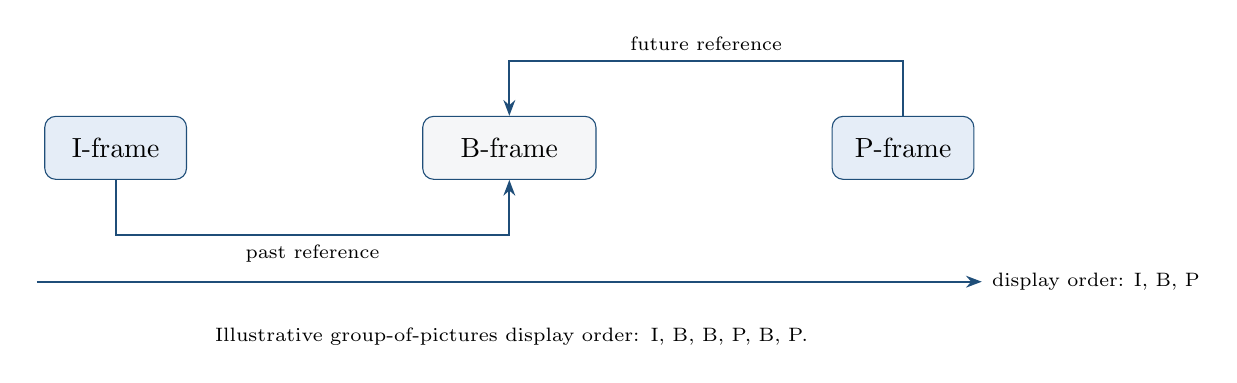
\begin{tikzpicture}[x=1cm,y=1cm]
\node[draw=navy,fill=paleBlue,rounded corners,minimum width=18mm,minimum height=8mm] (iframe) at (0,0) {I-frame};
\node[draw=navy,fill=paleGray,rounded corners,minimum width=22mm,minimum height=8mm] (bframe) at (5,0) {B-frame};
\node[draw=navy,fill=paleBlue,rounded corners,minimum width=18mm,minimum height=8mm] (pframe) at (10,0) {P-frame};
\draw[arrow] (iframe.south) -- ++(0,-0.7) -| node[pos=0.25,below,font=\scriptsize] {past reference} (bframe.south);
\draw[arrow] (pframe.north) -- ++(0,0.7) -| node[pos=0.25,above,font=\scriptsize] {future reference} (bframe.north);
\draw[arrow] (-1,-1.7)--(11,-1.7) node[right,font=\scriptsize] {display order: I, B, P};
\node[font=\scriptsize,align=center,text width=12cm] at (5,-2.4) {Illustrative group-of-pictures display order: I, B, B, P, B, P.};
\end{tikzpicture}}
\caption{B-frame prediction uses both a past I-frame and a future P-frame reference.}
\label{fig:ipb-reference}
\end{figure}

\topic{H.261}
H.261 targets low-delay videoconferencing at \(p\times64\) kbit/s with CIF/QCIF, 8x8 DCT, macroblocks, motion compensation, quantization, RLE, and variable-length coding; it uses I/P prediction.

\topic{MPEG}
MPEG serves storage/broadcast: MPEG-1 for CD video, MPEG-2 for DVD/TV, and later MPEG-4/H.264/HEVC for improved tools and rates. It supports I/P/B frames, flexible GOPs, and bidirectional prediction.

\topic{H.261 versus MPEG}
H.261 favors simpler, low-delay conversation; MPEG favors storage/broadcast compression, with B-frame delay and greater decoder complexity.

\begin{center}
\begin{tabularx}{\linewidth}{>{\bfseries}p{0.2\linewidth}XX}
\toprule
Aspect & H.261 & MPEG family\\
\midrule
Target & Low-delay videoconferencing & Storage, broadcast, and varied resolutions/applications\\
Rates/use & Approximately \(p\times64\) kbit/s; CIF/QCIF & MPEG-1 for CD-quality video; MPEG-2 for DVD/TV; later MPEG-4/H.264/HEVC and successors\\
Tools & 8x8 DCT, macroblocks, motion compensation, quantization, RLE, variable-length coding; I/P prediction & I/P/B frames, flexible/scalable GOP, bidirectional prediction, advanced motion compensation\\
Trade-off & Simpler prediction and low delay & Generally higher compression/quality potential; potentially more delay and decoder complexity\\
\bottomrule
\end{tabularx}
\end{center}

\end{document}
